\subsection{Overview...historically}
The tunneling effect describes the behavior of a particle that faces a potential barrier. In the classical picture the particle is prohibited to move across the potential barrier if its energy is lower than the barrier. In quantum mechanics, a wave character is added to the particle. When the wave now faces the potential barrier, a fraction of the wave package that constitutes the particle is transmitted through the barrier - an effect known as tunneling.

The tunneling effect was first observed by Hund in 1926 \cite{Mehra_tunneling_1982} in molecules, where he explained the sharing of an electron between atoms, each represented by a potential well. A principle fundamental for an understanding of covalent chemical binding. 

The first quantitative expression of the tunneling current in a metal-insulator-metal junction was introduced by Bardeen in 1961 \cite{Bardeen_tunneling_1961}. 

This lead to an early prototype build by Russell Young, John Ward and Fredric Scire in 1972. \cite{Young_topographiner_1972}. Here the basic principles of modern STMs is shown already (piezo movement, tunneling with metal tip). The concept was further improved so it gave rise to the first operational STM. It was build by Binning \& Rohrer in 1981 \cite{binning_tunneling_1982} where they were the first to report experimental evidence for the tunneling through an vaccum gap with controllable width. They showcased the excelled resolution capabilities by resolving the $7 \times 7$ reconstruction of the Si(111) surface \cite{binnig_1983}. They received the noble prize in 1986 \cite{_noble_price_1986} for "their design of the scanning tunneling microscope". The key features that allows for atomic resolution in STM is twofold. First the tunneling current diminishes quickly with increasing vacuum gap, allowing for experimental accessibility of the vacuum gap distance. Second, the tip position can be controlled with high accuracy on a continuous scale by the use of piezo elements. These ceramic materials show the piezoelectric effect \cite{Martin_Piezo_1972} by which their length is precisely controllable through an applied voltage.

In the following the tunneling process through a vacuum gap between a metallic tip and sample will be summarized and used as model system to describe the basic concept of one dimensional tunneling.

\subsection{Theory...on 1D tunneling at a single point}
\index{STM!One dimensional tunneling}

\begin{figure}[]\centering
	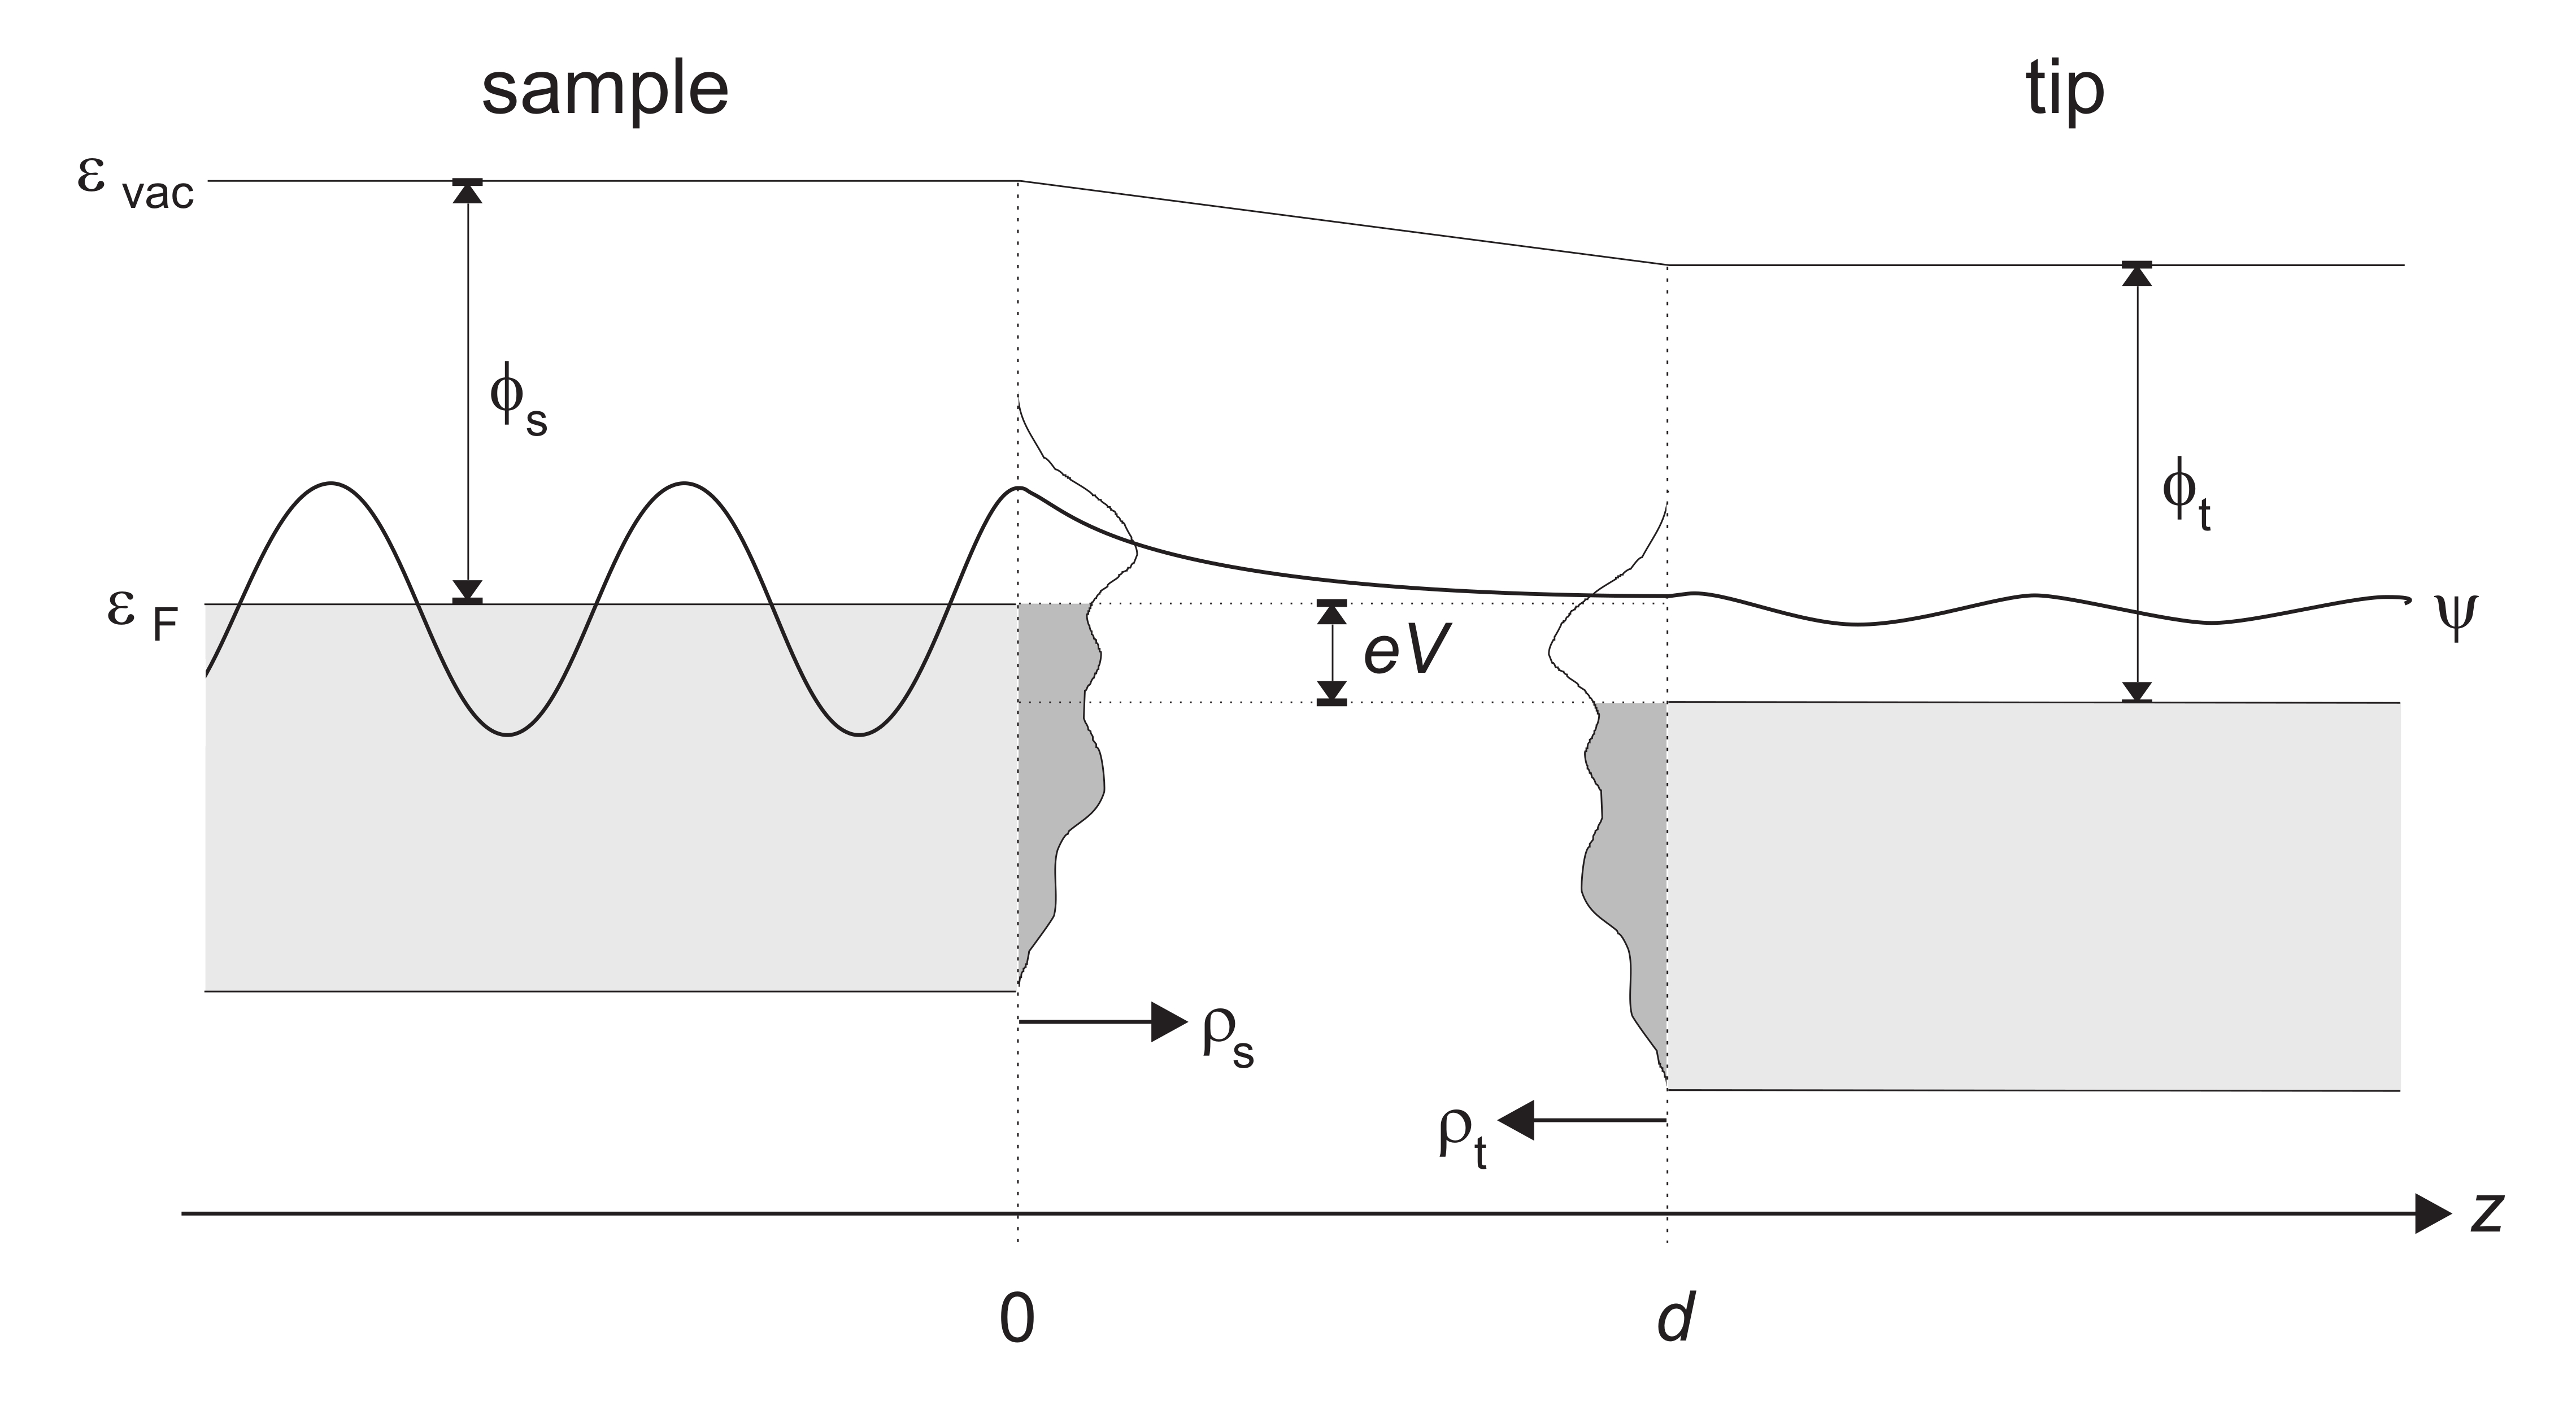
\includegraphics[width=0.7\textwidth]{./images/tunnel-barrier}
	\caption{Energy diagram to visualize the tunneling process between sample (left) and tip (right) separated by a distance d. Work functions of sample and tip ($\Phi_s$ and $\Phi_t$) separate the filled states (shaded regions) and the vacuum level ($\epsilon_{vac}$). Since sample ($\rho_s$) and tip DOS ($\rho_t$) may not be uniform, a fictional DOS is sketched in darker colors between both. The samples energy is lifted by $eV$ after a bias is applied and results in a net electron current from the sample into the tip. One tunneling process is indicated by a wave function in the sample. After overcoming the vacuum barrier its amplitude decreases and the corresponding electron occupies a free state (not shaded) in the tip material.  Taken from \cite{diss-schunack}}
	\label{fig:STM-barrier}
\end{figure}

While the tip (metal) is far away from the sample, their vacuum levels are the same. The corresponding Fermi energies of sample and tip lie below the vacuum level by the amount of their work functions ($\Phi_s$ and $\Phi_t$ for sample and tip respectively). Wave functions of electrons within the tip and sample decay exponentially in vacuum, depended on their energy with respect to the Fermi level.
If sample and tip are in thermodynamic equilibrium, their Fermi levels are the same. Electrons now face a potential barrier (approximately rectangular) which can be overcome if their energy is high enough and the barrier sufficiently narrow. When a voltage is applied across the tunneling barrier, the energy of the tip-electrons is shifted by $eV$ as illustrated in \autoref{fig:STM-barrier}. When a positive bias voltage is applied, electrons tunnel from the tip into unoccupied states in the sample - a negative bias results in a tunneling current in opposite direction. 

Following the model of \index{STM!Tersoff-Hamann} 
Tersoff-Hamann\footnote{Please's note that there are more models and 
corrections to them. An evolution from Bardeen's approach to the one done by 
Tersoff-Hamann can be found here \cite{lounis_theory_2014, 
wortmann_interpretation_2000} including Chen's expansion.}((1) uniform density of 
states in the tip, (2) temperature is low, (3) small bias voltage of some mV, 
(4) waveform of electrons in tip are s-waves) the tunneling current results to 
$$I=32\pi^3\hbar^{-1}e^2V\Phi_t^2 R^2\kappa^{-4}e^{-2\kappa R}\rho_t(E_F)\rho_s(r_o,E_F)$$ where $\rho_t$ is the density of states per unit volume of the tip, R the tip radius and $\rho_s(r_0,E_F)$ the Fermi level density of states in the sample\cite{bonnell_scanning_1993}. The distance between tip and sample is denoted as $Z$ and the inverse decay length of the electrons wave function is $\kappa=\frac{\sqrt{2m\Phi_t}}{\hbar}$. If $I$ is held constant one can see that the tip in principle follows a contour of constant Fermi level density of states at the sample surface, measured at the center of the curvature of the s-wave like tip. While its a good first approximation of the system, in many cases the bias is much higher than 10mV (\SIrange{1}{5}{\V}) so more than just the electrons near Fermi contribute. Also a uniform $\rho_t$ may not be accurate in all cases.

Using \index{STM!WKB} Wentzel-Kramers-Brillouin (WKB) theory\cite{wentzel_verallgemeinerung_1926, kramers_wellenmechanik_1926, brillouin_mecanique_1926} the tunneling current is given by
\begin{equation}
I=\int_0^{eV}\rho_s(r,E)\rho_t(r,eV+E)T(E,eV,r)dE
\label{WKB}
\end{equation}
where $\rho_s(\rho_t)$ is the density of states of the sample (tip) and T is the tunneling transmission probability
\begin{equation}
T(E,eV)=exp\left(-\frac{\textcolor{red}{\textbf{2}}Z\sqrt{2m}}{\hbar}\sqrt{\frac{\Phi_s+\Phi_t}{2}+\frac{eV}{2}-E}\right)
\label{Transmission-function} 
\end{equation}
If $eV<0$ the tunneling current is largest for $E=0$ (electrons on the Fermi-level of the sample), if $eV>0$ the tunneling current is largest for $E=eV$ (electrons of Fermi level in tip).

Due to the fact that the tunneling current is proportional the density of states in the tip and the molecule one can deduce the band structure within a range of several volts in the vicinity of the Fermi energy.

Since states with highest energy have the largest decay lengths in vacuum, most of the tunneling current is determined by electrons within close proximity to the Fermi level.\footnote{More information related to tunneling processes can be found here \cite{bonnell_scanning_1993}.}

\subsection{\textbf{S}canning \textbf{T}unneling \textbf{S}pectroscopy}
\paragraph{Theory...on STS}
\label{section:STS}
First changes of the tunneling current with the bias voltage were observed by Tromp et al. in 1986 \cite{tromp_atomic_1986}. They discovered a change in contrast when scanning a SI(111) surface with either positive or negative bias. The change in contrast is most apparent in semiconductors and semi metals\cite{bonnell_scanning_1993}, but adsorbates and charged areas of the sample change the DOS locally and therefore the contrast in STM. While simple results may be already obtained when comparing two images recorded at different voltages, more detailed information can be achieved. At low temperatures the vanishing lateral movement of molecules makes them also accessible to tunneling spectroscopy. It is possible to deduce the electronic configuration on with atomic spatial resolution.

Spectroscopic information (information on the DOS) can be obtained by either changing the bias voltage (I(V,z)-spectroscopy) or the tip-sample distance (V(z)-spectroscopy).  

Therefore the bias is modulated with a sinus like waveform. \index{STS!modulation}The frequency of the low amplitude modulation of the DC bias is much larger than the feedback loop frequency (\SIrange{1}{2}{\kilo \hertz}). The AC part of the tunneling signal is than recorded with a lock in amplifier. The in-phase component is directly the $dI/dV|_{V=V_{bias}}$, recorded simultaneously with the topography.\footnote{If the modulation frequency is too low, the feedback tries to compensate the modulation by changing the distance to the sample.	If the modulation frequency is too high, the capacitance between tip and sample leads to an $90\deg$ phase shifted current which increases with modulation frequency. One usually chooses the modulation frequency slightly above the cutoff frequency for the feedback loop.}

\index{STS!Bias below work function}
First let us consider small biases.
If tunneling conditions are such that $eV\leq\Phi$, observed features in $dI/dV$ are associated with the surface DOS. Critical points in the surface projected DOS give rise to features in $dI/dV$. Interpretation of these features with the WKB theory (i.e. differentiating equation \eqref{WKB}) gives
$$dI/dV=\rho_s(r,eV)\rho_t(r,0)T(\textcolor{red}{\textbf{eV}},eV,r)+\int_0^{eV}\rho_s(eV)\rho_t(r,E-eV)\frac{dT(E,eV,r)}{dV}dE$$
The first term contains the DOS of the sample and tip and the transmission function. While it is usually unknown, a closer look to \eqref{Transmission-function} indicates a smooth, monotonically increasing function in V. This mannered dependence on V gives a smooth background described by the second term $\int_0^{eV}\rho_s(eV)\rho_t(r,E-eV)\frac{dT(E,eV,r)}{dV}dE$.
Because T is smooth and monotonic the first term $\rho_s(r,eV)\rho_t(r,0)T(eV,eV,r)$ introduces the dependence on the DOS in the sample for energies $eV$ - our desired spectrum.

\subsection{...and how an image is created}
The current recorded in a certain area of the sample is translated into a contrast variation on a color scale. While some images encourage the operator to interpret points with high intensity as elevated atoms it is not that trivial. The \textbf{constant current mode}\index{STM:operating mode} is the most widely used one. The tip height is regulated with a feedback controller to achieve a constant tunneling current for the chosen bias. The recorded information is now the voltage applied to the z-piezo to maintain a plane with the same current. Sample features that increase the tunneling current cause the feedback to decrease it again by retracting the tip.

\subsection{Experimental details and machine description}
\paragraph{Experimental details}

\begin{itemize}
	\item[Topography images] show the change in z-direction to maintain the current set point
	\subitem Modified tip allows for real space imaging of molecular orbitals
	\item[dI/dV]
	\subitem single point (open feedback loop, sweeping bias): measure electronic properties – molecular orbital energies
	\subitem map (fixed bias, open feedback loop), show real space distribution of electronic states
\end{itemize}

\paragraph{Machine description}
Since all used UHV chambers have many common part, a typical setup is described with the LT-STM setup. Here the most experiments were carried out.
\begin{itemize}
	\item Commercial \textbf{Beetle-type STM scanner} \cite{zoephel_aufbau_2000}
	\subitem Three outer piezo tubes are used in slip-stick motion
	\subitem Moving on a helicoidal ramp is used to control height during tip approach (\SI{120}{\degree} segments, \SI{2}{\degree} inclination)
	\subitem TM tip attached to inner piezo tube used for lateral tip position, image width, scan speed, tip-sample distance
	\subitem Two dampling stages decouple the STM
	from the surrounding (Eddy current damping and floating on springs, floating chamber) (see experimental section below)
	\item \textbf{DSP controller}
	\subitem Measured tunneling current compared with set point
	\subitem Current to high => retract, current to low => approach => CC-mode
	\subitem Low pass filter for high frequency damping
	\item \textbf{Lock-In Amplifier}
	\subitem Used for STS measurements
	\subitem Sinusoidal modulation of bias voltage with a frequency higher than the low pass frequency of the DSP 
	\subitem Tunneling current modulated with the same frequency
	\subitem Differentiating (sin=>cos) is performed by reading the signal with a 90° phase shift (as sin and cos are shifted by 90°)
	\subitem Little noise and computing effort to achieve spectrum
	\subitem For Maps: DSP does not “recognize” modulation and change in current as topographic feature and regulates as without modulation
\end{itemize}

\paragraph{Vacuum system}

\paragraph{Cooling system} 
While low temperature (LT) STMs may be operated with solely helium, it is more resource-saving to cool the direct proximity of the sample and the STM with He, but to suppress the heat flow out of the He-cryostat with a second surrounding nitrogen cryostat (boiling point: \SI{77}{\K}, compare figure \ref{fig:STM-cryo}). This diminishes consumption of globally limited and rather expensive He. To maintain a temperature of \SIrange{5}{7}{\K}, one to two liters of liquid helium are required a day, plus an additional amount of three to four liters liquid nitrogen. Evaporated helium is reclaimed in a closed circuit with a system of purifying and storage/cooling steps so that only a small amount of helium escapes the circuit and is lost.

Sample temperatures down to \SIrange{5}{7}{\K} allow for observations not possible at elevated (room) temperature. Cooling not only reduces thermal drift in the piezo elements that are used to control the tip's position on the sample. Thermal energy at low temperature is not high enough for atoms or molecules to move on most substrates. Species mobile at room temperature (and therefor not representable at room temperature in the sub-ML regime) become immobile and accessible for ST microscopy and spectroscopy. STS spectra resolution is better at low temperatures as discussed in \ref{section:AFM-resolution}.

\begin{figure}[ht]\centering
	\subfigure[LT-STM setup mainly used in this work. Different functional groups are colored in different colors. A low base pressure in achieved with a combined pumping system comprised of ion pumps and turbo molecular pumps (cyan). The liquid helium/nitrogen bath cryostat (red) is used to maintain low temperatures. Sample holders are operated with a rote able, variable temperature manipulator. Sample preparation is done in a chamber (blue). After transfer to the LT-STM chamber (yellow) a gate valve is used to seal the LT-STM from remaining residual gas that may be present in the preparation chamber. Vibration isolation of the frame is achieved with legs floating on pressurized cylinders.]{
		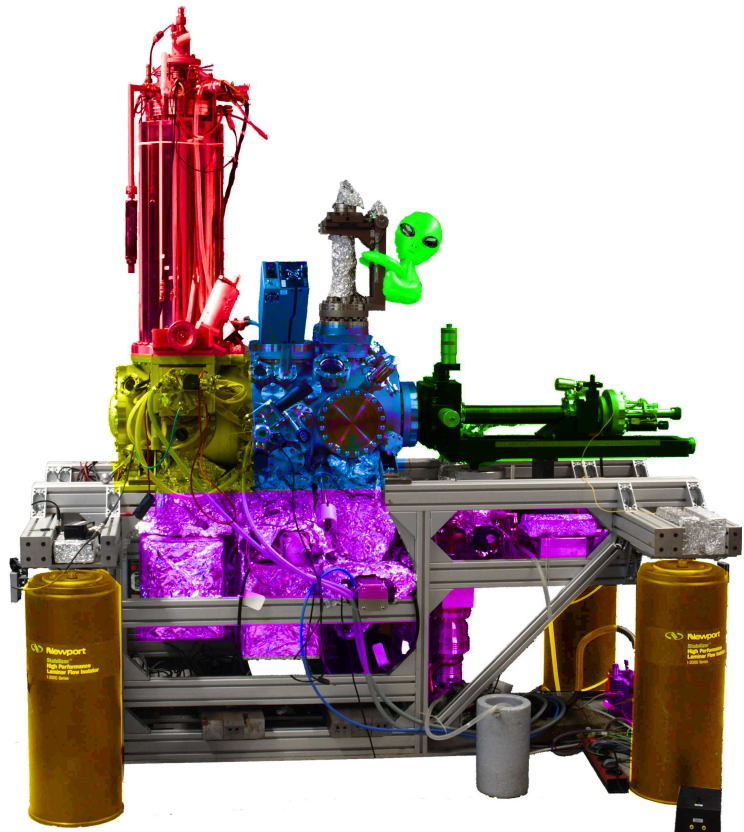
\includegraphics[width=0.45\textwidth]{./images/chamber-sketch.jpg}
		\label{fig:chamber-sketch}
	} \quad
	\subfigure[Scheme of a STM liquid bath cryostat. While in the inner measurement stage a temperature of $\approx \SIrange{5}{7}{\K}$ is achieved with a liquid helium reservoir, an outer liquid nitrogen cryostat is used to isolate the evacuated inner cryostat from the surrounding room temperature.]{
		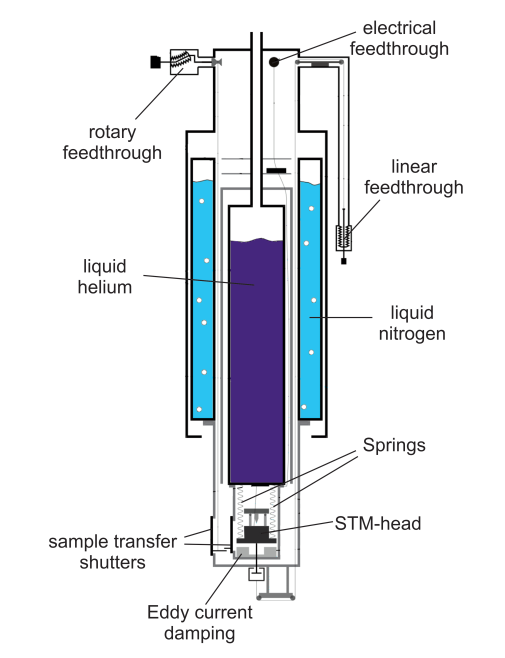
\includegraphics[width=0.45\textwidth]{./images/sketch-cryo.jpg}
		\label{fig:STM-cryo}
	}
	\caption{Typical setup for low temperature measurements. A vibration isolated UHV chamber is used to prepare samples and investigate them in a separable chamber with either STM or AFM. A liquid bath cryostat is used to maintain low temperatures. Images stem from {diss-knud}}
	\label{fig:STM}
\end{figure}

\paragraph{Damping stages}
Two damping stages are used, one for the chamber and a separate one for the STM.
\begin{itemize}
	\item The whole UHV system is placed on air pressurized legs. These can be elevated on demand, so that the chamber floats on four dampers and external vibrations/shocks are damped.
	\item A second stage decouples the sensitive STM from the rest of the setup. First the complete STM stage hangs on springs to further limit the direct influence of vibrations. Second the remaining oscillation amplitude is damped by a eddy current damping. It is made of three magnets in close proximity to the surrounding support so that eddy currents are induced for each minute movement. The eddy current is typically larger at cryogenic temperatures, that results in a damping that works best at low temperatures. The kinetic energy of the oscillating system is transferred by the eddy currents into heat within the surrounding conductor. The heat is then mitigated by the external cooling of the cryostat.
\end{itemize}

\paragraph{Piezo elements}
\begin{wrapfigure}{O}{5cm} \centering
	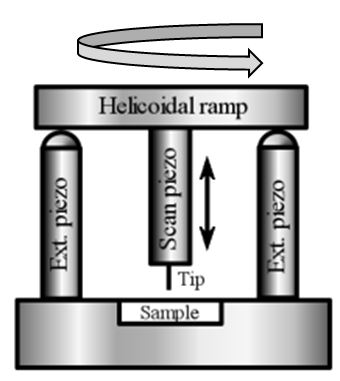
\includegraphics[width=5cm]{./images/STM-sketch-2}
	\caption{STM sample stage to control the tips position. The coarse movement is controlled by exterior piezos. Each move up/down on a heliocoidal ramp with slip-stick motion. The precise scanning is done with a central piezo to which the tip is attached. Taken from}
	\label{fig:stm-heliocoidal ramp}
\end{wrapfigure}
The position of the tip (x, y, z) is controlled with a set of piezos (see \autoref{fig:STM-tip}). In this work a tubular piezo stack is used to control the tips position with a central piezo element located on top of the tip. The piezo length can be controlled with the voltage applied to them, which is used to choose not only the tip-sample distance, but other parameters like image size and scan speed as well. All of these parameters are monitored with the STM software. A feedback loop controls the piezo voltages. For recording an image the area is raster scanned in consecutive lines, applying a sawtooth voltage to the fast scan direction. The next lines are chosen by slowly increasing the voltage along the slow scan direction. Depending on the operating mode the tip-sample distance is controlled by piezo elements, too.

%\begin{figure}[ht]
%	\begin{center}
%	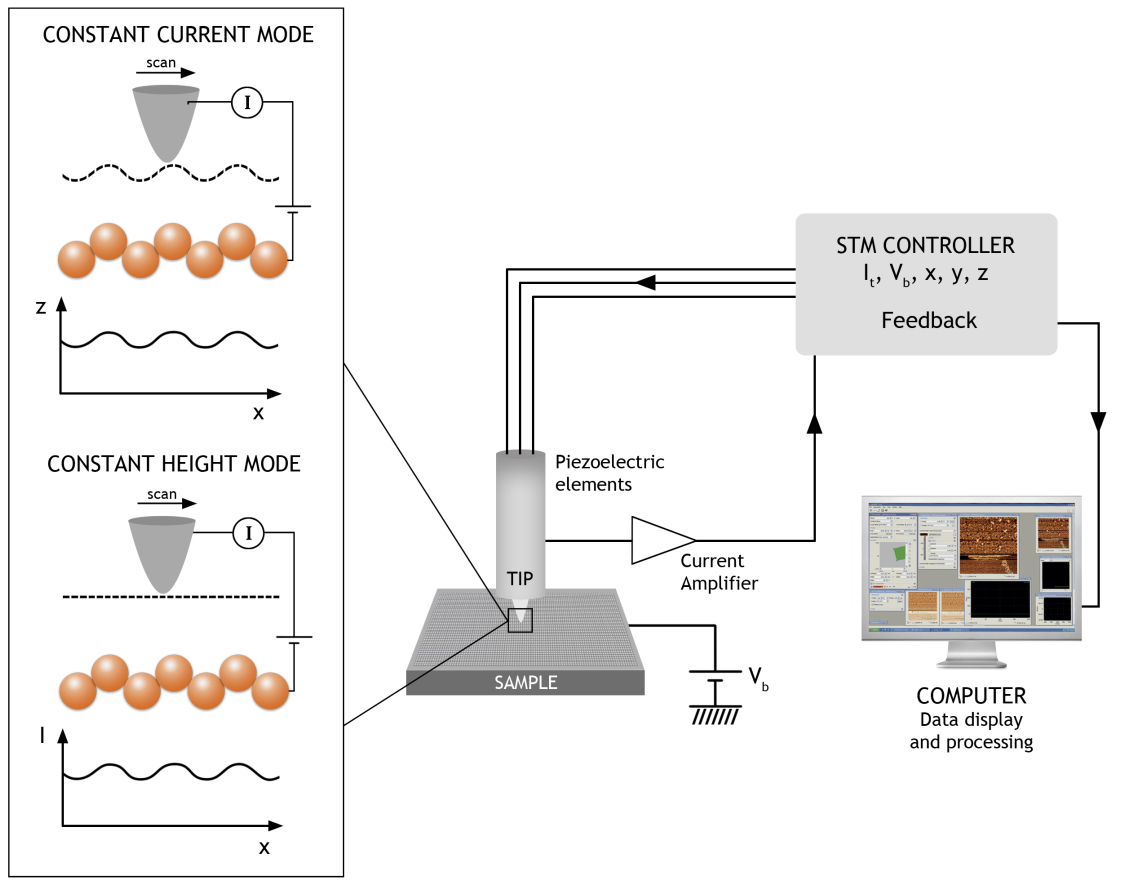
\includegraphics[width=0.45\textwidth]{./images/STM-sketch}
%	\end{center}
%	\caption{Taken from \cite{diss-manuela}}
%\end{figure}

\begin{figure}\centering
	
\subfigure[]{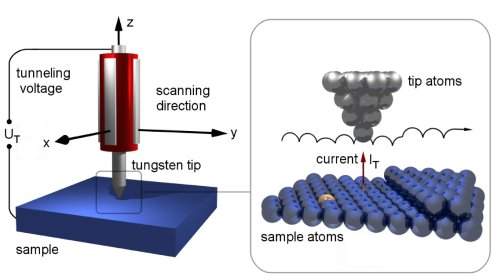
\includegraphics[width=0.6\textwidth]{./images/stm-rutgers-modified.jpg}\label{fig:STM-tip}}
	
\subfigure[]{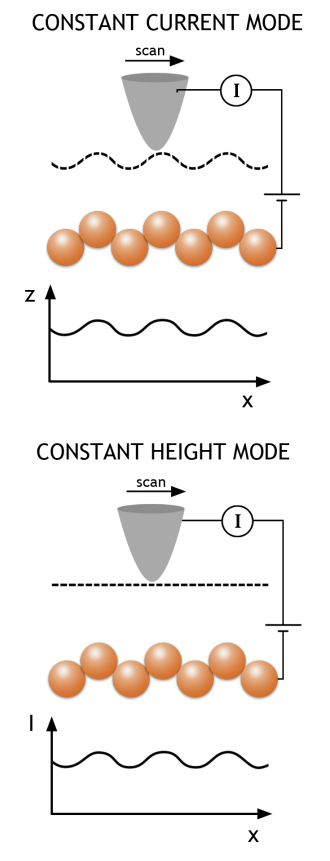
\includegraphics[height=0.33\textwidth]{./images/STM-sketch-cut}
\label{fig:STM-modes}}
	\caption{Operating principles of an STM. \subref{fig:STM-tip} A macroscopic sketch  shows the central piezo that controls the tip position above the sample. A microscopic sketch shows the tips movement in constant current mode while moving across a atomic step edge. The main piezo is divided in four parts to control movement in the x-y plane and tip-sample distance\cite{STM-rutgers}. \subref{fig:STM-modes} The difference between constant current and constant height mode. While the tip follows the samples LDOS in constant current mode (top) the tip height remains constant in constant height mode (bottom). Taken from \cite{diss-manuela}.}
	\label{fig:STM-sketch}
\end{figure}


. Tunneling current between tip and sample depends on the LDOS of tip and surface and is therefore not implicitly maximized at the atomic positions. It may also vary with the bias voltage applied in a non-trivial manner. Investigation of this behavior led to the establishment of a new measurement technique, called scanning tunneling spectroscopy (see \autoref{section:STS}). 

\subsection{Limitations}\index{STM:resolution}The accuracy of a STM is very high with spatial resolution down to the atomic scale. Due to the fact that the tips motion is controlled with different piezos, one has to take different elongations in different directions into account. For example, if the STM scans the fast scanning direction just a bit further than the slow scan direction, the resulting image (although pixel wise square) is no longer physically square anymore. Imagine a square (1:1 side ratio, diagonal angle 45\textdegree) where one side is elongated by 5\%. The resulting square (1:1.05 side ratio, diagonal angle 43.6\textdegree) looks square because it has the equal number of pixels in both directions, but it is physically rectangular. The expression used to calculate the uncertainty with known calibration parameters is
$$\Delta \Theta = 45 - \frac{180}{\pi}\cdot\arctan(\frac{1}{1+x})$$ where x is the percentage of one side being longer. This results in an uncertainty of 0.3\textdegree(1\%), 1.4\textdegree(5\%, see example above), 2.7\textdegree(10\%). For moderate shear, conformity is almost conserved and the uncertainty below 2\textdegree.

Mechanical and thermal vibrations limit the resolution of the STM, too. Therefor several damping stages decouple the STM from the surrounding. Although STM works at room temperature, additional cooling may be applied to reduce the thermal vibrations.

Because STM is sensible to electronic changes, it may change the footprint of an adsorbed compound \cite{sautet_interpretation_1992}. When laterally approaching an adsorbate this results in an additional tunneling current, because now electrons do not only tunnel directly into the substrate but through the adsorbate as well. Interferences between both tunneling processes depend on the adsorbate's orbital-symmetry and tip-shape. Local density of states calculations \cite{tersoff_theory_1985, lang_theory_1986, eigler_imaging_1991} is not adapted to grasp this effect since the tip is considered far away from the surface. Moreover, the tip radius or the tip-substrate distance is optimized to fit the lateral size of the adsorbate print with the experimental image \cite{tersoff_theory_1985, eigler_imaging_1991}.

\begin{itemize}
	\item Mechanical and thermal vibrations limit the resolution of the STM \& STS
	\item No chemical resolution
	\subitem XPS used for chemical identification of adsorbates
\end{itemize}

